\documentclass{article}
\usepackage{explorations}

\title{Introduction}
\module{Module 0}
\course{Explorations I}

\begin{document}
\begin{notes}
  Start with the following video: \url{https://youtu.be/gvQNybQO6E4}
\end{notes}

\section*{A New Way of Learning Mathematics}

\begin{wrapfigure}[27]{R}{0.25\textwidth}
  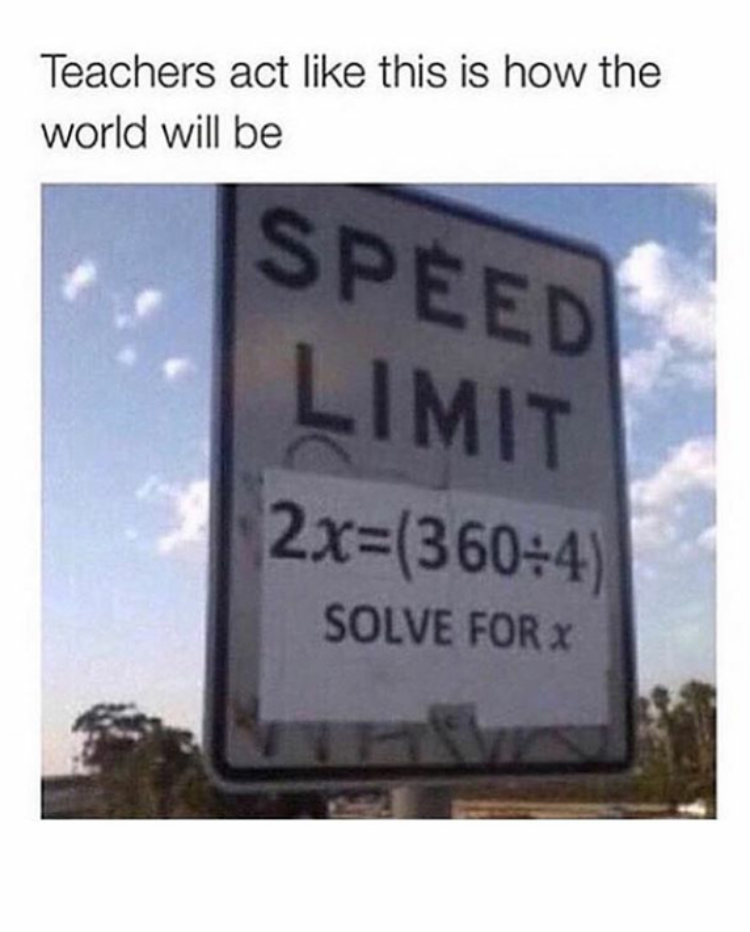
\includegraphics[width=0.25\textwidth]{speedlimit.png}

  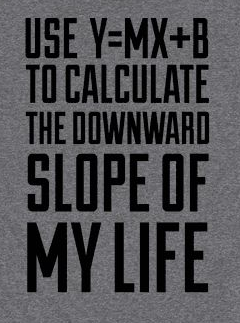
\includegraphics[width=0.25\textwidth]{downwardslope.png}
\end{wrapfigure} 

For many students, mathematics does not bring happy memories or feelings. Some even dread learning mathematics. One important question is why do so many students dislike a subject that Gauss called the “Queen of all Sciences.” 

Many say how important mathematics is, and how it is used to understand the world around us through many different fields. Some say mathematics is a universal language and that humans are hardwired to do basic mathematics.


Yet many struggle and come to associate this subject with negative feelings. Most never attain an appreciation for how mathematics is used in their day-to-day lives.  We are asking every student who has decided to take this course to let go of their past experiences, their erroneous belief that they are “bad at Math” or that they do not have a “Math brain,” and definitely let go of their ego and pride. 

It does not matter what level you are at, Mathematics will always have challenges for the mind. There is an inherent challenging nature in this discipline, and it is in this struggle that you are indeed actually learning. In such struggles, you are developing different analytical skills and are increasing your neuroplasticity, that is literally making your brain grow. Such a realization is a very important step in dealing with this subject. 

Our curriculum is intended to generate thought-provoking questions, analytical reasoning, critical thinking, and most of all, an appreciation and realization for the need and even desire to improve such skills. You will be developing into a more effective thinker and a more informed member of our 21st century society.   Throughout this course, the way you will be exposed to mathematics will be very different than in a traditional algebra curriculum.  The purpose of this approach is for the student to identify with the subject matter and to gain a sense of intellectual curiosity, and therefore motivate the learning process.

We will introduce ways of doing problems that at times may look very different from how you may have learned them in the past. At times this could even seem more difficult or unconventional, but the intention is for you to focus on your thought process, rather than on just trying to get a “correct” answer to a problem.  Because students prefer taking courses where content is relevant and engaging, this approach to learning mathematics is intended for the student to deeply explore the subject matter. We expect to receive your feedback throughout the course.  So, please communicate with your instructor anything that you would like to discuss about the structure and content presented.

\section*{Module 0: Appreciating Mathematical Beauty}

There are many things that affect people’s views about their ability and their likes or dislikes of any subject. For some, an aversion to mathematics begins in elementary school when they are first exposed to fractions.  Early failures in a math class, or in-class punishments or embarrassing moments in front of peers, or having to learn what seems like meaningless procedures that detract from creative thinking, are all experiences that can stay with some students for years.  In some cultures, parents and peers maintain norms that math is hard or even unnecessary. In other cultures, girls more than boys, learn to question their mathematical ability. 

It is difficult to identify a single cause for a dislike, anxiety, or negative self-view that developed over many years.  One thing is for sure: ABSOLUTELY and without exception --- even to the most evolved and gifted minds --- mathematics will eventually challenge you to the point where you end up feeling that you hit a massive wall and thus continuing to improve in learning it seems just impossible.  There are mathematical problems so incredibly complicated, that to this day remain unsolved.  So, do not judge yourself by your ability to actually get a correct answer quickly, but by your resilience in continuing to systematically devote meaningful time, energy and struggle in your studies.  \emph{\textbf{If you are truly struggling, then you are definitely learning.}}

It is at this point that a growth mindset, a gritty attitude, and a persevering disposition are absolute necessities. For without this, that “wall-hitting” experience that you feel in the subject will grow even deeper and more unrelenting.  However, with a self-advocate and positive attitude, it is very possible to overcome such feelings and modify these thoughts.  Without exception, EVERY mathematician has at some point felt this feeling of doubt and struggle in this subject.  We all have our strengths and weaknesses. However, as human beings we can also develop new skills and abilities through diligence, practice, tenacity, positivity, grit and becoming conscious of our thought processes.

\begin{wrapfigure}[14]{R}{.35\textwidth}
  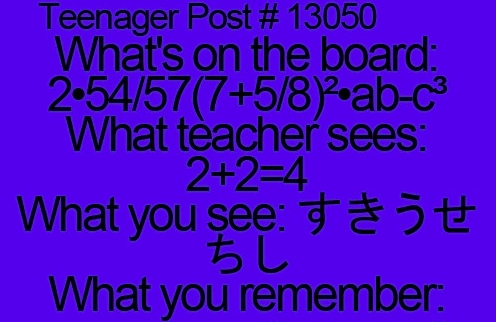
\includegraphics[width=.35\textwidth]{whatteachersees.png}

  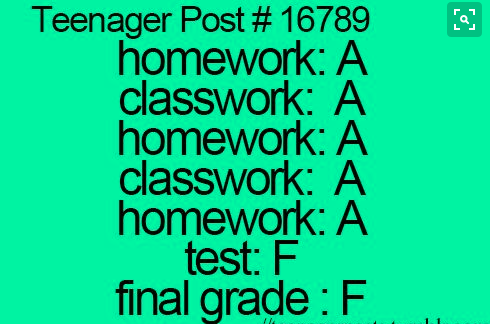
\includegraphics[width=0.35\textwidth]{grades.png}
\end{wrapfigure}
\begin{description}
\item[Goals:]
  \begin{itemize}
  \item[]
  \item Promote student self-reflection about the subject matter
  \item Promote a clear and specific plan for success in the math course as well as for the student’s academic and professional goals
  \item To maintain this plan of action in the forefront with every student, thereby making them responsible for their own learning and academic experiences.
  \end{itemize}
\end{description}

Write a two to three-page typed, double-spaced essay about your personal math history.

\begin{notes}
  This is to be turned in by the end of the first week of the semester.  Have the students begin coming up with ideas for this first written assignment. Please specify your presentation requirements for the essays.
\end{notes}

Address the following:
\begin{itemize}
\item What is your mindset about mathematics?
\item What math courses and teachers do you particularly remember most and why?
\item Describe a positive and a negative math experiences you have had, and what did you learn about yourself through these experiences.
\item What are your academic and professional goals, and explain how your life has brought you to have such goals and what role do you think math would play in achieving these goals?
\item What do you think you currently need to be able to reach these goals and how do you intend to make these goals your reality?
\item Describe in ample detail and being very specific what will you do to succeed in this course.
\end{itemize}

Make a pact with yourself on doing all that you have stated in your essay and perform weekly or bi-weekly evaluations on your progress.  If you do feel anxiety while taking math tests or doing math problems, pay careful attention to your biography and strategize on how you will overcome challenging experiences. In your history, there may be some anxiety-provoking events that may surface. Once you finish looking at any negative math-related events from your past, put them away. Put away any self-views such as “I am just bad at math.” We don’t believe in a victim-complex in mathematics, but we do believe that we are the creators of our future. Start with a fresh attitude and a new approach.  You will see how even mathematics can be rewarding and even fun to explore, like for our blue jay friend in the right!

\begin{notes}

  Show these videos on the first day of class.  Each video is between 6--9 minutes.  Pause to have a discussion between these two videos.
  
  \begin{itemize}
  \item Angela Duckworth --- Grit: \url{https://youtu.be/H14bBuluwB8}
  \item Mathematigal --- Fear of dealing with Math: \url{https://youtu.be/Xs9aGVUZ3YA}
\end{itemize}

\end{notes}

\begin{notes}
  Here is where you need to set a new perspective for students.  The video links below can help you bring about this new perspective.  The perspective here is to value and encourage critical and analytical thinking.  This approach to teaching Math hinges on exploring math topics where the process is more important than some correct answer.  In this class, we encourage that a significant part of the course grade be geared to the student’s effort in critical thinking, and the explanations from the students to justify their reasoning on a problem.  

Students put an over-emphasis on grades and GPA, especially the many students that are on a transfer track.   Here is where you as the instructor need to both balance the process taken AND the student’s explanation, with the correct answer to a problem.  Here is where you need to show them how valuable it is to struggle while doing mathematics, because their ability to learn future topics grows significantly.  

After discussing this first activity with the students and having them write down some ideas on how they will address the questions posed by this writing assignment, show them the following video:

How you can be good at Math By Jo Boaler (TED Talk Stanford): \url{https://youtu.be/3icoSeGqQtY}

You should go thru the entire video. It has quite a bit of information for both students and instructors.  This video exemplifies what SDCC Math department is looking to create in this way of doing mathematics.
\end{notes}

\begin{notes}
  For the following three links below you may want to consider some of the following activities or assignments.  

Assign these next 2 videos for the next class session.  At the beginning of the second class you will have the students work in groups of 3. If there is one person left over, make a final group of four, and if there are two students left over, let them be a group on their own.  Have the students discuss what new perspective they gained with regards to doing math by watching these videos.  Have the students come up with 6 – 8 tangible things that they both learned about what it takes to learn math and how they will incorporate these strategies into this math course and future ones.

\url{https://youtu.be/smHZNr5qOb0} (Angela Duckworth – University of Pennsylvania Talk) 

\vspace{0.25in}

\url{https://youtu.be/mHQ_0ehnavI} (What it’s like to study Mathematics in College) 

For this video, among the main points is that a student HAS to be self-advocate AND they network to help themselves learn math.  All students build into their study time, working in groups and working in a Tutorial Center.
\end{notes}

\begin{notes}
  Or for this video, have the students write a one page essay on how this video can relate to learning mathematics, and what does each student think is the most important factors for them in learning mathematics based on the premises of this video and have the students read their essays in class.

\url{https://youtu.be/LNHBMFCzznE} (Dr. Lara Boyd – Your Brain Will Never Be The Same When You Learn Anything – Neuroplasticity) 
\end{notes}

\clearpage

\textbf{Homework due next class:  \hfill Name: \underline{\hspace{2in}}}

\textbf{Watch the following video. Write down 3 things you liked or learned from it. Be ready to discuss it in class.}

\href{https://youtu.be/3icoSeGqQtY}{\emph{How You Can Be Good at Math}} by Jo Boaler.
\begin{description}
\item[URL] \url{https://youtu.be/3icoSeGqQtY}
\item[QR Code] \qrcode{https://youtu.be/3icoSeGqQtY} 
\end{description}

\vspace{0.25in}

\begin{enumerate}[label=\textbf{\arabic*.}]
\item \

  \vfill
  
\item \

  \vfill
  
\item \

  \vfill
  
\end{enumerate}
\end{document}

%%% Local Variables:
%%% mode: latex
%%% TeX-master: t
%%% End:
